\chapter{第二教学楼}

%\renewcommand\thefootnote{\roman{footnote}}

清华园目前有六个公共教学楼,其中一教、二教都位于早期建筑群处。

% TODO: 来张图瞧瞧

越老的建筑,常常就有越多的迷,二教也不例外,这栋楼几乎是园子里故事最传奇的地方。
二教远离宿舍区和现在以三四五六教为核心的教学区,虽说往常白天的时候也有许多游客,但游客也不会进入教学楼,因此其实没有什么人气;
而且二教不开放自习,没课的时候也就显得格外冷清。
不过由于楼内都是大教室,因此有课的时候二教的教室也显得比别处的教室空旷;
又开着空调,即使是酷暑,在二教里也会觉得冷。当然这一点上,六教也差不多,冷气开得一个比一个足。

二教最让人不解的地方莫过于教室的编号和分布了。
这里教室的楼层号并没有单独编号,而是顺着一教往下编的。一教一共三层,因此二教的教室全部都在“四层”。
而且二教从结构上看明明可以设置四个大教室,但实际上却只有401、402和403三个教室,因此留下了找不到的404这样的传说。
此外,二教的三个教室还要从三个不同的门进入:401从南门,402要走东边的正门,403则要从北门进去再上楼。
简而言之,二教的结构和布置透露着难以言明的诡异。

不寻常的地方自然就会有不寻常的故事,二教闹鬼的传说也因着其奇特的设置不胫而走了。
据说曾有一对女生在咖啡厅赶死线,半夜两点赶完活儿之后回寝,路过早已静楼完毕大门紧锁的二教时,突然听到楼内传来一阵急促的敲门声,受到了极大的惊吓。
照理来说,晚上十一点的时候所有的教学楼就都要静楼锁门了,保卫不大可能把谁漏在楼里;更何况二教平日里根本不开放自习,一下课保卫就把人全轰走了,更不可能有人滞留在内。那么如果不是保卫失职的话,就只能是闹鬼了。
鉴于这起事件是发生在新世纪的,有人就猜测会不会是六教的小男孩被关在了里面。然而二教和六教也颇有些距离,那六教的小男孩一直趁傍晚在六教活动,真的会跑到老远外的二教这里来吗?
因此就又有人猜想,可能是之前的冤魂没有驱干净。

这就说到了二教一个流传甚广的传说了。
七七事变后日本侵略者占领了清华园,将当时多处校内建筑占用为军事设施。
45年日本人战败后,清华园光复。次年,清华师生也从昆明迁回了清华园。
然而相传原址复课后,二教却发生了许多古怪的事情。
最先是402的一盏灯变成了“长明灯”,无论如何也无法熄灭;
后来楼梯上也开始无来由地渗出血液,地下室也时常传来凄惨的哭声;
甚至上课的时候,黑板上还会浮现出怎么也擦不掉的鬼脸。
这事儿逐渐惊动了校方,于是校方特意从白云观请了道士来捉鬼。
传闻讲那道士一到二校门就觉得二教的阴气很重,进了二教之后发觉问题出在地下室。
一行人进了地下室后,道士作法,撒下石灰,发现地面上凭空出现了一串脚印,顺着脚印就发现墙上有一个堵死的门洞。那门洞封得很仔细,不留意看的话根本瞧不出来。
设法破开那道墙后,出现了一段阴森曲折的地道,地道的房间里堆满了白骨。这差不多就是闹鬼的源头了。
后来又从地道里搜出了许多细菌实验设备,这才知道这里曾被日本侵略者用作人体实验室。
据说在北平沦陷的八年里,有数千位同胞在此受尽折磨,被残忍杀害;而日本人仓促撤退时来不及完全销毁证据,于是封死了他们挖出的地道,妄图掩盖他们的罪行,却不曾想数千冤魂终于还是曝光了这地道中曾发生的惨案。
这之后,二教的地下室就封死了;而且为了增些阳气,疏导些阴气,二教的南北两侧又开了两扇门,据称是取“三阳开泰”之意。
而二教的楼层号从“4”编起,也不是为了和一教接续上,而是在地下室封死之前,算上了地下的层数来数的,后来地下室封死之后,也没有再改。

只是这个故事也有些年代了,而且那之后的几十年里也没有在传出新的闹鬼事件,因而很多人觉得,那敲门声应该与此无关。
关于敲门声从何而来的争论,最终也不了了之,最后不少人也都相信,可能只是受坊间二教鬼故事的影响,两人过于紧张了,出现了错觉。
此事便是这样。

不过说到二教奇特的楼层编号方式,除了那“地下室说”之外,还有种“空中楼阁说”。
次说认为,二教原先是和一教一体的,就在一教的顶上,因此楼层号也就顺着一教来编了。
但是后来有高人说工字厅有紫气,东边这一块地一直空着会让紫气外泄,不若在这里再建一座楼堵住外泄的紫气。
然而其时校内资金不足以另起新楼,故又请了大师行移山填海之术,将原一教顶层的几间阶梯教室移到了空地上,然后另开了几个门,是为现在的二教。
刚移好时,二教和一教的联系还没有断,顺着二教一层向下的楼梯还能走回到一教的三层;又由于二教下面并无地基,故被称作“空中楼阁”。
后来学校将原一教、二教之间的楼梯拆掉,封死了一教楼顶和二教地面,一教和二教从此便不能再直接联通了。

\begin{figure}[!t]
	\centering
	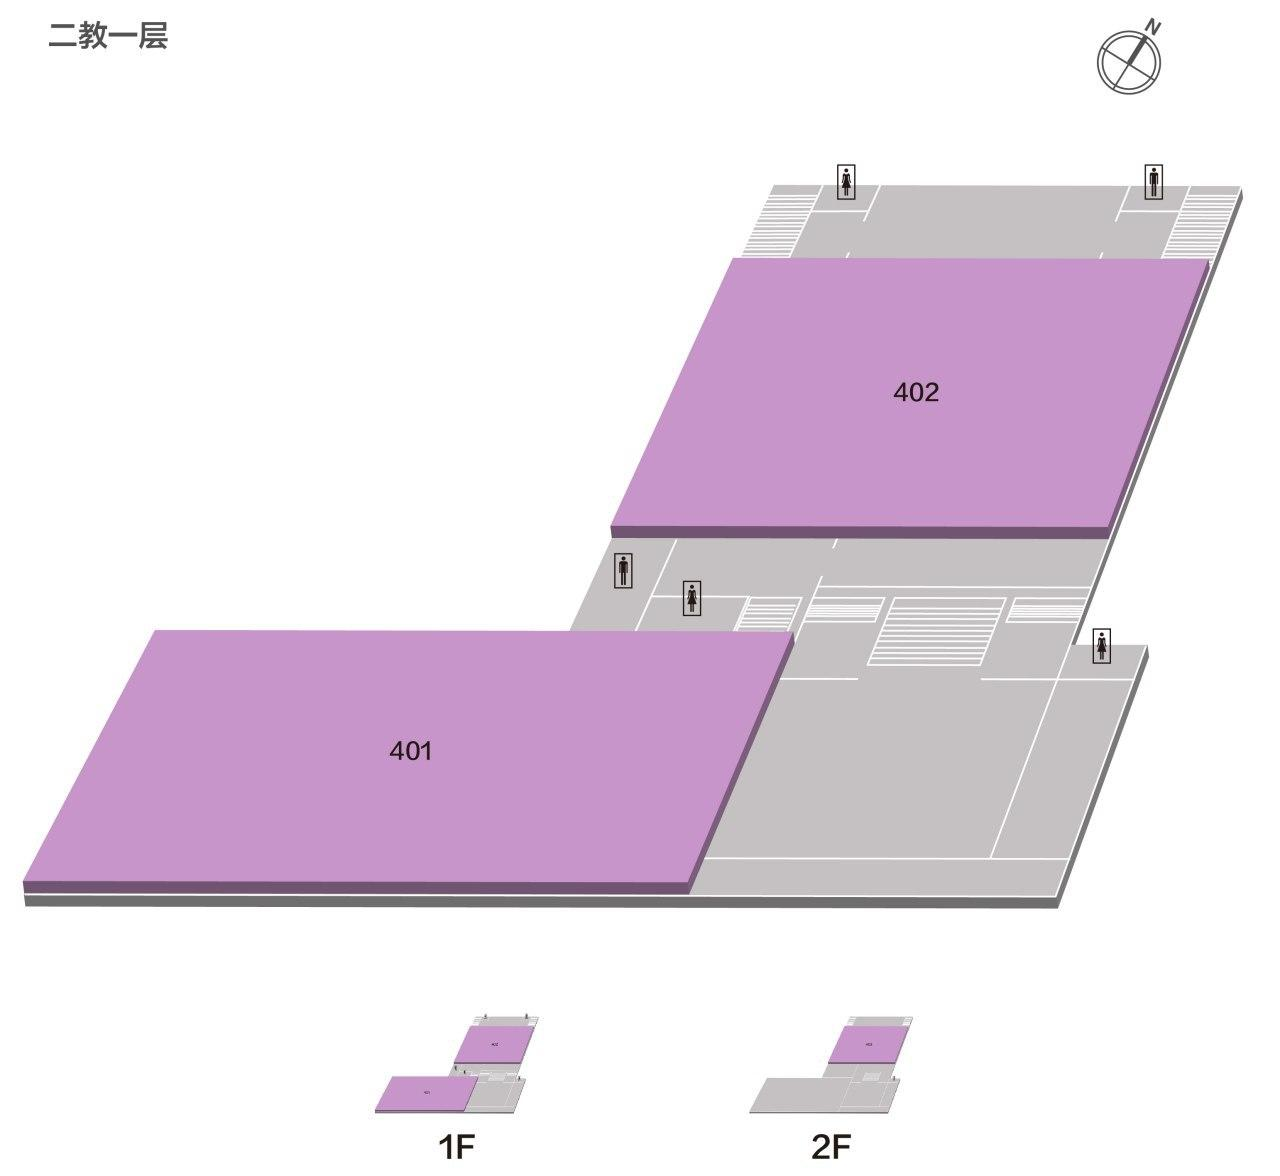
\includegraphics[width=\linewidth]{figures/二教一层.jpg}
	第二教学楼一层结构。两张结构图都取自清华大学“学在清华”公众号2018年9月16日的推送\href{https://mp.weixin.qq.com/s/SHW-wviq3NYemcHZBRgi5w}{《解救路痴 | 清华教室最强指南》}。
\end{figure}

\vfill

\paragraph{闲谈}
笔者记得自己在大一的时候在校内的某公众号上看到过一篇推送,做的是清华园校内怪谈集锦。感觉这种奇闻异事应该是又“小五爷园”来发的,不过近来回去搜索历史却并没有搜到相关的文章。想来也有可能是什么群里发出来的链接被笔者看去了吧。
看完之后印象最深的就是二教地下室的传说,因此这番也打算围绕着二教来写。只是当时看的故事如今早已模糊不清,故又到网上搜集了些材料,在此转述出来。

\begin{figure}[!t]
	\centering
	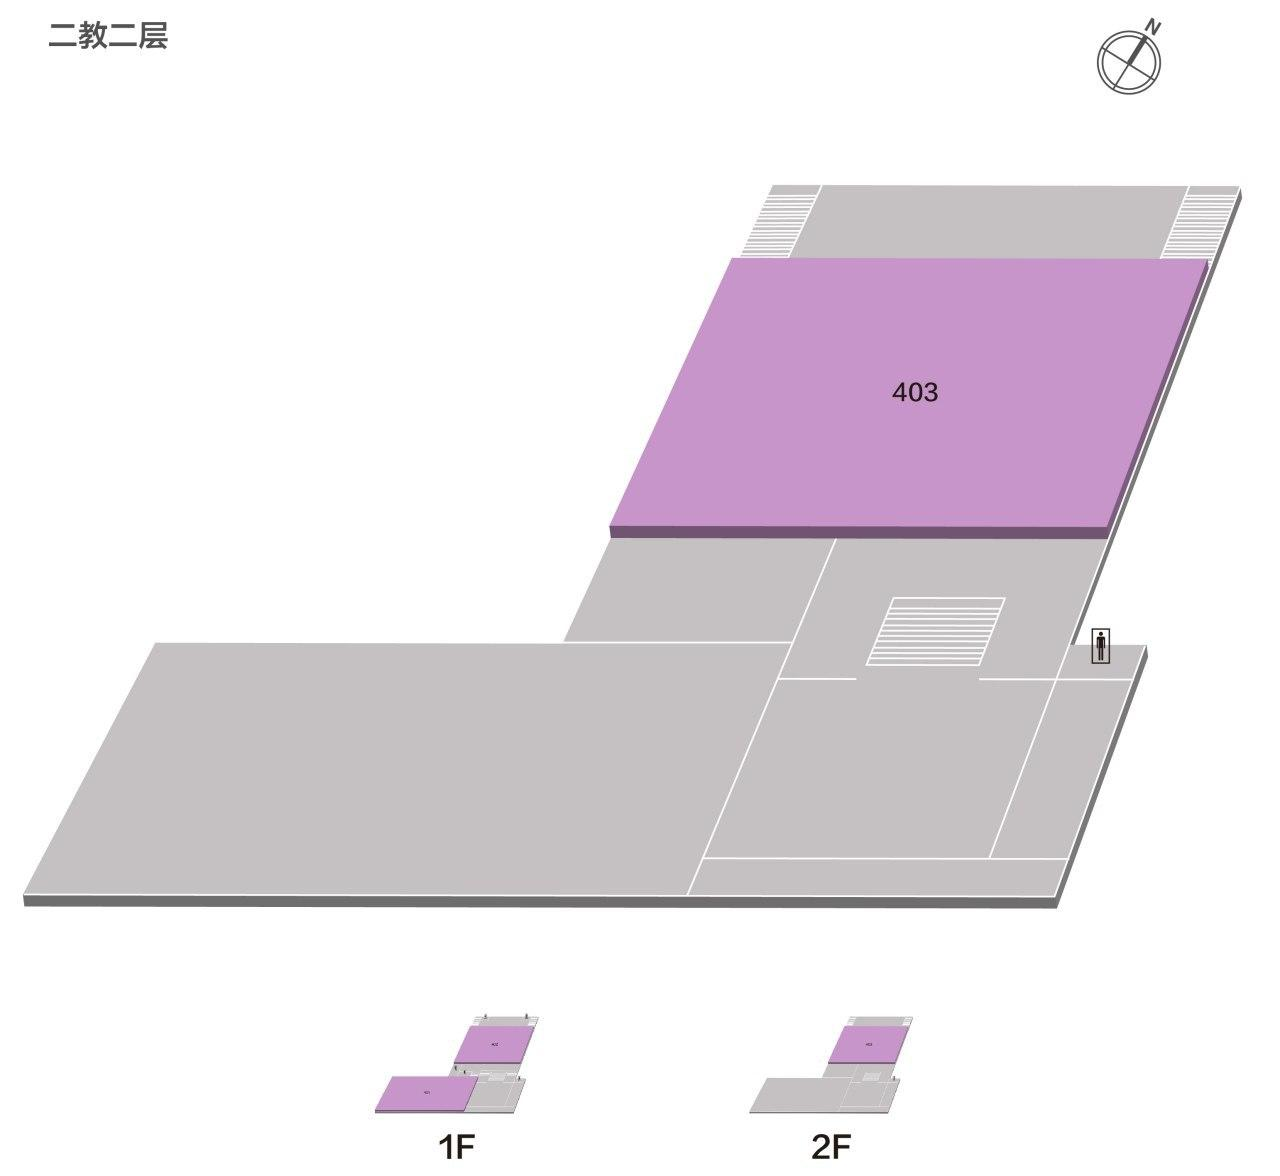
\includegraphics[width=\linewidth]{figures/二教二层.jpg}
	第二教学楼二层结构
\end{figure}

说到二教,其实笔者在二教只上过两门课。
大一下的时候上安宇老师的《大学物理(1)》,线上慕课加线下习题讨论课,每周的习题讨论课就是在二教的403。
403在二楼,从二教的北门进去,上楼梯就是403的后门。记得那是403的前门往里是不开的,貌似是堵死的,出入只能走后门,而且二教也不开放自习,给人感觉很神秘。
之后大二下,罗予频老师的《计算机原理与应用》也是在二教,不过是在402。402就在403的楼下,可以从北楼门由教室后门进,也可以从正楼门由教室前门进。
网上谣传401只能从南门进,但笔者记得当时401和402的前门差不多就对着,从正门是可以进去的。二教的南门笔者也没仔细留意过,感觉好像这个门是不开的吧。
二教的结构图上401的楼上,大概就是传说中404的位置。看维基百科上的介绍说,二教其实是三个教室和一个会议室,所以404的位置可能就是会议室吧。这一点笔者也不确定,从来没有从正门处的楼梯上过二楼,403的前门也出不去,因此不知道那个位置是什么样子的。
404这个编号也很巧,正好是HTTP协议中“资源未找到”(Page Not Found)错误的代码,因此校内也流传着“二教404 Not Found”这个梗儿。

根据公开的校史信息,目前校内六座公共教学楼里,最早建设的第一教学楼落成于1952年,而第二教学楼则建成于1954年,都在建国后,因此日本人实验室的故事毫无疑问是伪造的。
不过日本人的人体实验室大约也并非空穴来风。有些记载显示,侵华日军占领清华园期间,曾占用过图书馆老馆做军事医院,二教这个传说的来源可能与此有关。
此外,在搜集材料的时候,还看到有人提起说,文革期间二教确实发生过一些什么事情,但是笔者却没有找到更详细的记述。
话说到人体实验室,在现在校内西北门西侧,医学院那篇区域,靠近学校边界的一个小角落里,有一排平房,是学校的人体实验室,以前阳光长跑的时候,笔者和J君曾胡碰乱撞跑到过这里。

此外,二教好像是没有地下室的,更不会有地道之类的。
倒是大礼堂的地下,建得很深,还很曲折,仿佛地宫一样。
虽然现在只是个厕所,但不知道过去是不是有考虑过用于防空之类的。

还有一个有趣的事情。
清华的一教到五教的牌子上写的都是“第几教\textbf{学}楼”,而六教的牌子上写的却是“第六教\textbf{室}楼”,并不一致。

有人曾务实地分析二教不开放自习的原因,猜测应该是这里离教学区、宿舍区、食堂都很远,来这里自习的时空成本很高,因此来的人少;二教又是阶梯教室,不适合自习,于是就只开放了一教和清华学堂,而没有开放二教。笔者亦以为然。
说到这里,笔者还曾遇到过某个死脑筋在一教自习的人。
笔者大四时选了个课,是后八周的课。周五早上去一教102上课的时候,总能看到个人在那里自习,然后等到7点50多快上课的时候,就会收拾东西离开。
笔者在这里就不去探究为何要大清早的跑到离宿舍区老远的一教来自习了,而是讨论下另一件事情。
按理来说,上过几周课之后,榆木脑袋用它的朽木脚趾也能想到,一教102周五第一节是有课的,为什么仍然要死脑筋地就在一教102早自习而不能换间教室呢?这个人一直到最后一周的周五都保持着这种令人迷惑的行为,即不知道什么时候,总之很早就来到一教102自习,然后等到7点50多教室里快要上课的时候再离开。笔者想不通。

园子老了,就会有各种各样的故事,清华园的怪谈也不仅仅局限于第二教学楼,其他神秘的、有故事的地方也还有很多,比方说,二教对面的清华学堂。
就笔者的个人感觉来说,清华学堂实在比二教更加阴冷。笔者就去过几次清华学堂,最早是C君引笔者进去转了一圈;后来是大四试选了叉院的《密码学基础》,在那里上了几周课,后来退了。每次进去都觉得——很冷,即使是夏天,也会觉得浑身发冷;冬天便更甚,总觉得仿佛没有开暖风一样。实在不敢想象C君他们学堂班的同学是怎么在里面上过四年的课的。
再一个流传甚广的传说之地就是六教了。传闻六教是建在乱葬岗上的,结果去年六角北边的出土文献保护中心和新土木馆的施工地点还真挖出了明清古墓,也堪称传奇了。
还有传闻说六教东边的什么第十三个杨树的异闻的。顺便一提,据说六教东边、主楼后边、综体前边的这片小树林,平时就是鸳鸯夜戏的地方,不过笔者没有亲自考证过。
网上还流传万泉河乃阴气之源,而28号楼南侧,横跨万泉河的那座小桥处——其实就是之前小桥烧烤的地方——是阴气汇集之地,故设置了小桥烧烤店,引入些烟火气,驱驱阴气。
不过如今小桥烧烤也拆除这么久了,好像也没有发生什么鬼魅害人的事件。
笔者还看到有人提及主楼425也有些奇异的传说,不过笔者没有找到具体的故事,故在此不表。

\nocite{ClassroomBuilding2_Leg1,ClassroomBuilding2_Leg2,ClassroomBuilding2_Info1_THU,ClassroomBuilding2_Info2_Wikipedia,ClassroomBuilding2_Anal1,ClassroomBuilding6_Leg1,WanquanRiver_Leg1}
\putbib
